%
\section{Application: Stochastic Submodular Maximization} 
\label{sec:stochastic-maximization}
%

As our first application, consider the sensor placement problem
introduced in \secref{sec:intro}.  Suppose we would like to monitor a
spatial phenomenon such as temperature in a building.  We discretize
the environment into a set $\groundset$ of locations.  We would like
to pick a subset $A\subseteq\groundset$ of $k$ locations that is most
``informative'', where we use a set function $\hat{f}(A)$ 
to quantify the informativeness of placement $A$. \citet{krause07nearoptimal} show that many natural objective functions (such as reduction in predictive uncertainty measured in terms of Shannon entropy with conditionally independent observations) are monotone submodular. 

%
Now consider the problem,
where the informativeness of a sensor is unknown before deployment (e.g., when deploying cameras for surveillance, the location of objects and their associated occlusions may not be known in advance, or varying amounts of noise may reduce the sensing range). We can model this extension
by assigning a state $\rlz(\elem)\in\outcomes$ to each
possible location, indicating the extent to which a sensor placed at location
$\elem$ is working.  To quantify the value of a set of sensor deployments
under a realization $\rlz$ indicating to what extent the various
sensors are working, we first define $(\elem,{\outcome})$ for each $\elem \in \groundset$ and $\outcome
\in \outcomes$, which represents the placement of a sensor 
at location $\elem$ which is in state 
$\outcome$.  We then suppose there is a function 
$\hat{f}:2^{\groundset\times\outcomes} \to \NonNegativeReals$ which
quantifies the informativeness of a set of sensor deployments in arbitrary
states.  (Note $\hat{f}$ is a set function taking a set of (sensor
deployment, state) pairs as input.) 
The utility $f(A,\rlz)$ of placing sensors at the locations in $A$
under realization $\rlz$ is then
$$f(A,\rlz) := \hat{f}(\set{(\elem,\rlz(\elem)) : \elem \in A}).$$ 
\ignore{
 \begin{figure}%
 \centering 
 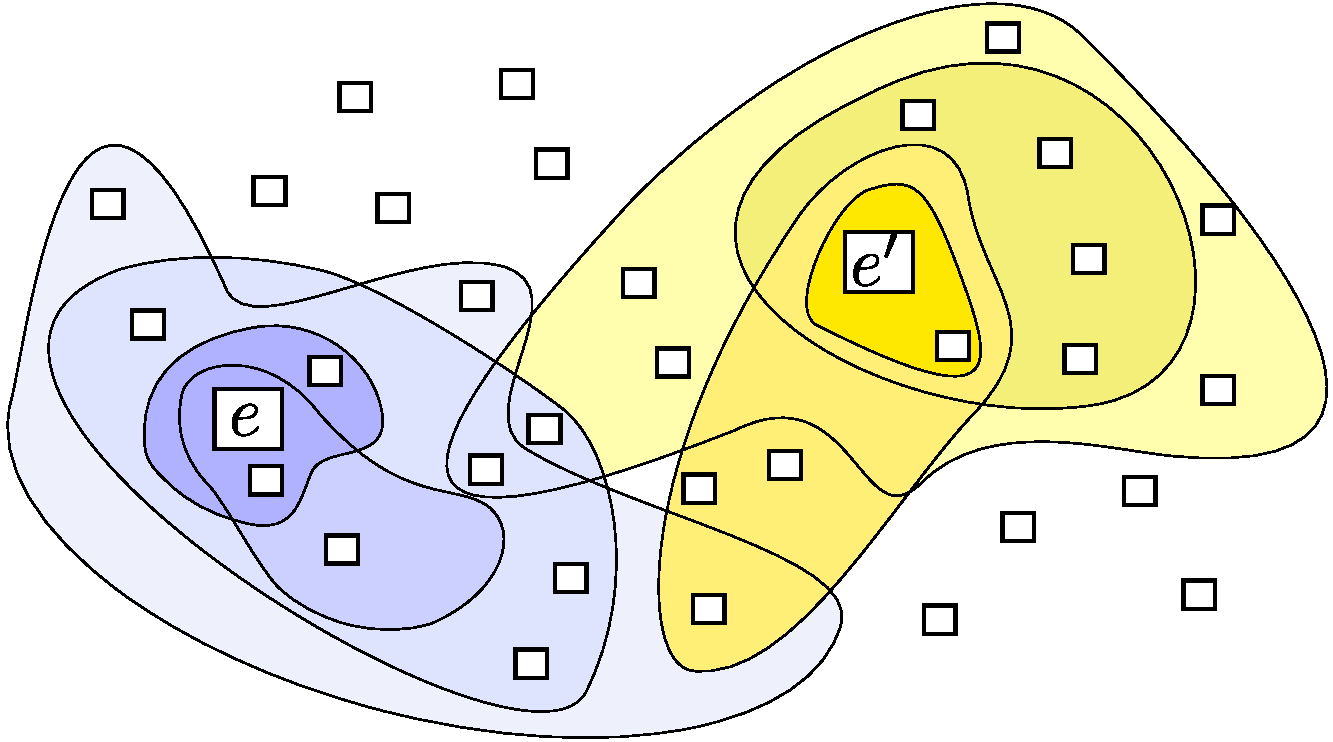
\includegraphics[height=4.5cm]{figs/stocSetCover}
 \caption{Illustration of part of a Stochastic Set Cover instance.  Shown are
   the supports of two distributions over sets, indexed by items $e$ (marked in blue) and $e'$ (yellow).   \label{fig:stocsetcover}}
 \end{figure}
}
\looseness -1 We aim to adaptively place $k$ sensors to maximize our expected utility.
We assume that sensor failures at each location are independent of each other, i.e., 
$\prob{\rvrlz = \rlz}=\prod_{\elem \in \groundset}\prob{\rvrlz(\elem) = \rlz(\elem)},$
where $\prob{\rlz(\elem)=\outcome}$ is the probability that a sensor
placed at location $\elem$ will be in state $\outcome$. 
\citet{AsadpourNS08} studied 
a special case of our problem,  
in which sensors either fail completely (in which case they
contribute no value at all) or work perfectly,
under the name \emph{\probname}. They proved that the adaptive greedy
algorithm obtains a 
$(1-1/e)$ approximation to the
optimal adaptive policy, provided $\hat{f}$ is monotone submodular.  
%
%
We extend their result to multiple types of failures
by showing that $f(A,\rlz)$ is \term submodular with respect to distribution $\rlzprior$ and then invoking Theorem~\ref{thm:max-cover}. \figref{fig:stocsetcover} illustrates an instance of Stochastic Submodular Maximization where $f(A,\rlz)$ is the cardinality of union of sets index by $A$ and parameterized by $\rlz$.

\begin{theorem}  \label{thm:WINE}
Fix a prior such that 
$\prob{\rvrlz = \rlz}=\prod_{\elem \in \groundset}\prob{\rvrlz(\elem) = \rlz(\elem)}$
and an integer $\budget$,
and let the objective function 
$\hat{f}:2^{\groundset\times\outcomes} \to \NonNegativeReals$ 
be monotone submodular.  
Let $\policy$ be any $\alpha$-approximate greedy policy attempting to maximize $f$, 
and let $\policy^*$ be any policy.  Then 
for all positive
integers $\ell$,
\[
\avgf(\prune{\policy}{\ell}) \ge \paren{1 - e^{-\ell/\alpha k}}
\avgf(\prune{\policy^*}{k}) 
\mbox{.}
\]
In particular, if $\policy$ is the greedy policy (i.e., $\alpha = 1$) and $\ell = k$, then
$\avgf(\prune{\policy}{k}) \ge \paren{1 - \frac{1}{e}} \avgf(\prune{\policy^*}{k}).$%
\end{theorem}

\begin{proof}
We prove Theorem~\ref{thm:WINE} by first proving $f$ is \term monotone
and \term submodular in
this model, and then applying Theorem~\ref{thm:max-cover}.
\Term monotonicity is readily proved after observing that 
$f(\cdot, \rlz)$ is monotone for each $\rlz$. 
Moving on to \term submodularity, fix any $\prlz, \prlz'$ such that 
$\prlz \subseteq \prlz'$ and any $\elem \notin \dom(\prlz')$.
We aim to show $\diff{\prlz'}{\elem} \le \diff{\prlz}{\elem}$.
Intuitively, this is clear, as $\diff{\prlz'}{\elem}$ is the expected marginal
benefit of adding $\elem$ to a larger base set than
is the case with $\diff{\prlz}{\elem}$, namely  $\dom(\prlz')$ as
compared to $\dom(\prlz)$, and the realizations are independent.
To prove it rigorously, 
we define a coupled distribution $\mu$ over pairs of realizations $\rlz \sim
\prlz$ and $\rlz' \sim \prlz'$ such that 
$\rlz(e') = \rlz'(e')$ for all $e' \notin \dom(\prlz')$.
Formally, 
$\mu(\rlz, \rlz') = \prod_{e \in \groundset \setminus
  \dom(\prlz)}\Pr{\rvrlz(e) = \rlz(e)}$
%
if  $\rlz \sim \prlz$, $\rlz' \sim \prlz'$, and $\rlz(e') =
\rlz'(e')$ for all $e' \notin \dom(\prlz')$; 
otherwise $\mu(\rlz, \rlz') = 0$.  
(Note that $\mu(\rlz, \rlz') > 0$ implies $\rlz(e') = \rlz'(e')$ for all $e' \in \dom(\prlz)$ as well,
since $\rlz \sim \prlz$, $\rlz' \sim \prlz'$, and  $\prlz \subseteq \prlz'$.)
Also note that $\rlzmass{\rlz \mid \prlz} = \sum_{\rlz'} \mu(\rlz, \rlz')$ and $\rlzmass{\rlz' \mid \prlz'} = \sum_{\rlz} \mu(\rlz, \rlz')$. 
Calculating 
$\diff{\prlz'}{\elem}$ and $\diff{\prlz}{\elem}$ using $\mu$, we see 
that for any $(\rlz, \rlz')$ in the support of $\mu$, 
\begin{eqnarray*}
  \label{eq:1mc}
f(\dom(\prlz') \cup \set{e}, \rlz') - f(\dom(\prlz'),
  \rlz')  & = & \hat{f}(\prlz' \cup \set{(\elem,\rlz'(\elem))}) -
  \hat{f}(\prlz'))\\
 & \le & \hat{f}(\prlz \cup \set{(\elem,\rlz(\elem))}) -
  \hat{f}(\prlz)) \\
 & = & f(\dom(\prlz) \cup \set{e}, \rlz) - f(\dom(\prlz),
  \rlz)
\end{eqnarray*}
from the submodularity of $\hat{f}$.
Hence 
\[
\begin{array}{lllll}
  \label{eq:2mc}
\diff{\prlz'}{\elem} & = & \sum_{(\rlz, \rlz')} \mu(\rlz, \rlz') \paren{
f(\dom(\prlz') \cup \set{\elem}, \rlz') - f(\dom(\prlz'),
  \rlz')} &  & \\[3mm]
  & \le & \sum_{(\rlz, \rlz')} \mu(\rlz, \rlz') \paren{ f(\dom(\prlz) \cup \set{\elem}, \rlz) - f(\dom(\prlz),
  \rlz)} & = & \diff{\prlz}{\elem}
\end{array}
\]
\ignore{
\begin{eqnarray*}
  \label{eq:2mc}
\diff{\prlz'}{\elem} & = & \sum_{(\rlz, \rlz')} \mu(\rlz, \rlz') \paren{
f(\dom(\prlz') \cup \set{e}, \rlz') - f(\dom(\prlz'),
  \rlz')} \\
  & \le & \sum_{(\rlz, \rlz')} \mu(\rlz, \rlz') \paren{ f(\dom(\prlz) \cup \set{e}, \rlz) - f(\dom(\prlz),
  \rlz)}\\
 & = & \diff{\prlz}{\elem}
\end{eqnarray*}
} %
which completes the proof. 
\end{proof}






%
%
%
%
%

